\documentclass{article}
\usepackage[utf8]{inputenc}
\usepackage[T1]{fontenc}
\usepackage{listings}
\usepackage{xcolor}
\usepackage{geometry}
\usepackage{amsmath,amsfonts,stmaryrd,amssymb}
\usepackage{enumerate}
\usepackage{helvet}
\usepackage{algpseudocode}
\usepackage{hyperref}
\usepackage[compact]{titlesec}
\usepackage{csquotes}
\usepackage{authblk}
\usepackage{tikz}

\hypersetup{
    colorlinks=true,
    linkcolor=blue,
    filecolor=magenta,      
    urlcolor=cyan,
    pdftitle={Overleaf Example},
    pdfpagemode=FullScreen,
}
\usetikzlibrary{arrows.meta,chains,positioning}

\titlespacing{\section}{0pt}{*0}{*0}
\titlespacing{\subsection}{0pt}{*0}{*0}
\titlespacing{\subsubsection}{0pt}{*0}{*0}

\geometry{
        paper=letterpaper,
        top=2.5cm,
        bottom=3cm,
        left=2.5cm,
        right=2.5cm,
        headheight=14pt,
        footskip=1.5cm,
        headsep=1.2cm,
        %showframe,
}

\definecolor{codegreen}{rgb}{0,0.6,0}
\definecolor{codegray}{rgb}{0.5,0.5,0.5}
\definecolor{codepurple}{rgb}{0.58,0,0.82}
\definecolor{backcolour}{rgb}{0.95,0.95,0.92}

\lstdefinestyle{mystyle}{
    backgroundcolor=\color{backcolour},   
    commentstyle=\color{codegreen},
    keywordstyle=\color{magenta},
    numberstyle=\tiny\color{codegray},
    stringstyle=\color{codepurple},
    basicstyle=\ttfamily\footnotesize,
    breakatwhitespace=false,         
    breaklines=true,                 
    captionpos=b,                    
    keepspaces=true,                 
    numbers=left,                    
    numbersep=5pt,                  
    showspaces=false,                
    showstringspaces=false,
    showtabs=false,                  
    tabsize=2
}

\lstset{style=mystyle}

\title{Procedurally Generated Tower Defense 3D}
\author[1]{Tori Broadnax}
\author[1]{Jeffrey Do}
\author[1]{Richard Roberts}
\author[1]{Minh Vu}
\affil[1]{George Mason University}

\setlength{\parskip}{\baselineskip}
\setlength{\parindent}{0pt}
\begin{document}
\maketitle

\begin{abstract}
    The overall goal of this project was to create a 3D tower defense game that has procedurally generated levels. The report is broken up into four primary sections: \hyperref[sec:Requirements]{Requirements}, \hyperref[sec:Technologies]{Technologies}, \hyperref[sec:Timeline]{Timeline}, and \hyperref[sec:Reflection]{Reflection}. In the requirements section, we will be quoting mostly from the Project Proposal--you do not need to reference it because enough context will be provided. We will identify what was planned to do, what was accomplished, how it was accomplished, and what was failed to accomplish. In the technology section, we will describe what technologies were used and how they aided us. Additionally, we will describe what parts beyond that given technology were implemented by us. The timeline section will chronologically detail what steps we took to reach our final product. Lastly, the reflection section will be individualized and it will specify what each group member contributed, challenges he/she/they faced, and any other personal notes.
\end{abstract}

\newpage

\tableofcontents

\newpage

\section{Requirements}
\label{sec:Requirements}

\subsection{Procedurally Generated Level}
\label{Procedurally Generated Level}

\begin{displayquote}
    \small
    The tower defense level will be procedurally generated. There should be at least one path from the enemy spawn to the tower. The tower will be placed randomly. There should be tiles that cannot have weapons placed on them (like trees), and tiles that can. Weapons should not be able to be placed on the path.
\end{displayquote}

This was the primary requirement of the project, and it was the most difficult to implement. The initial stages of the algorithm were kind of atrocious looking back on it. The algorithm then, and still, currently only works for a ten by ten grid/map size. The basis of this algorithm is that a start and endpoint would be generated. The start would be where enemies spawn, and the end would be where the tower is or the enemies' goal. A depth-first search would then be conducted and start until it found the endpoint, it would then set all the tiles that it cross to get to that path to be a value of "walkable".

\vspace{5mm}

\begin{algorithmic}
    \Procedure{generate-map}{$map$}
    \State $start \gets (0, \Call{random}{map.size.y})$
    \State $end \gets (map.size.y - 1, \Call{random}{map.size.y})$
    \State \Call{depth-first-search}{$start, end$}
    \EndProcedure
\end{algorithmic}

The problem with the algorithm was that it would produce a path that would be touching itself, making it uninteresting and kind of illogical. Additionally, there would be no way for the enemy to traverse this path in an "attractive" manner most of the time. The solution was to implement something nodal pathfinding using A*. The concept is that we would choose a set of waypoints and pass them into A* so that it would produce an optimal path between them.

\vspace{5mm}

\begin{algorithmic}
    \Procedure{generate-map}{$map$}
    \State $start \gets (0, \Call{random}{map.size.y})$
    \State $end \gets (map.size.y - 1, \Call{random}{map.size.y})$
    \State $waypoints \gets \emptyset$
    \State \Call{set-add}{$waypoints, start$}
    \For{$i \gets 3, i < 7, i = i + 2$}
    \State $pos \gets (i, \Call{random}{map.size.y})$
    \State \Call{set-add}{$waypoints, pos$}
    \EndFor
    \State \Call{set-add}{$waypoints, end$}
    \For{$i \gets 0$}
    \State \Call{find-path}{$waypoints[i], waypoints[i + 1]$}
    \EndFor
    \EndProcedure
\end{algorithmic}

This solution proved to work well. It, in addition to some other neighbor choosing filtering algorithm, allowed the paths to look much more natural and interesting. The \lstinline{FindPath} method adds the nodes produced by A* to an array that enemies can access to use when navigating themselves. Most if not all of this is done in \lstinline{GenerateMap.cs}.

\subsection{User Interface}

\begin{displayquote}
    \small
    There should be a tower health indicator. There should be a menu for selecting weapons to build. Once selected, the player should be able to select a tile, and the weapon should build if funds are sufficient. There should be a currency indicator. There should be buttons for starting and stopping the movement of enemies (like a pause).
\end{displayquote}

The tower health indicator is placed on the main UI and referred to as the player's health. There are three buttons present for selecting between the ballista, cannon, and blaster. The currency indicator is placed on the same menu as the health. When an enemy dies, the currency indicator will be increased. When the player builds a weapon, the currency will decrease. The game will pause when \lstinline{ESC} or \lstinline{P} are pressed.

\subsection{Weapons}

\begin{displayquote}
    \small
    There should be multiple types of weapons that vary in damage, rate of fire, and range. Weapons will fire projectiles at enemies in their range. The player should be able to build these weapons on tiles in exchange for currency.
\end{displayquote}

There are three types of weapons: the ballista, cannon, and blaster. They each have different damages, rates of fire, ranges, and projectile types. When a weapon is selected for building, hovering over a green grass tile will turn it yellow, indicating that the weapon can be built on that tile. Tiles that do not highlight in yellow indicate that they cannot be built on.

\subsection{Enemies}

\begin{displayquote}
    \small
    Enemies will have pathfinding towards to tower. When enemies reach the tower, a corresponding tower health deduction should take place. Enemies will have varying health, speed, and currency drops. Enemies should detect collisions with projectiles and take damage from them.
\end{displayquote}

There are two types of enemies: green ufo and purple ufo. These enemies have different amounts of health, speed, currency drops, and damage. Enemies have a health bar indicator above them, and when the health reaches zero they will be destroyed. Upon reaching the tower with health left, it will deal damage to the player.

\subsection{Reach Requirements}

\begin{itemize}
    \item Upgradable Weapons
    \item Weapon Selling
\end{itemize}

Both of these reach requirements were not met. For both of these items, a menu would have to appear when the weapon is clicked showing various buttons to upgrade or sell. We did not have the time to allocate toward making this UI element so we focused efforts elsewhere. The weapon selling would be relatively simple, just destroy the game object, the upgrade weapons part would not. It would require additional 3D assets and more game balancing.

\section{Technologies}
\label{sec:Technologies}

\begin{itemize}
    \item Unity
    \item Kenney Tower Defense
\end{itemize}

Unity was the game engine that was used to create this game. It aided a lot in the placement of models and the UI. However, all of the procedural generation was done via script manually, and the engine did not do this. A* was also manually implemented in scripts. Some other items that were done by scripts are linking all the components together, allowing them to seamlessly interact with one another. The base view for the game is simply an empty screen--there are no models in view (only UI elements); only when you click the play button do you see items appear. \hyperref[sec:References]{Kenney Tower Defense} is a 3D asset pack with the essentials to get started with making a 3D tower defense game. Making 3D assets goes beyond the scope of this class so we avoided custom assets.

\section{Timeline}
\label{sec:Timeline}
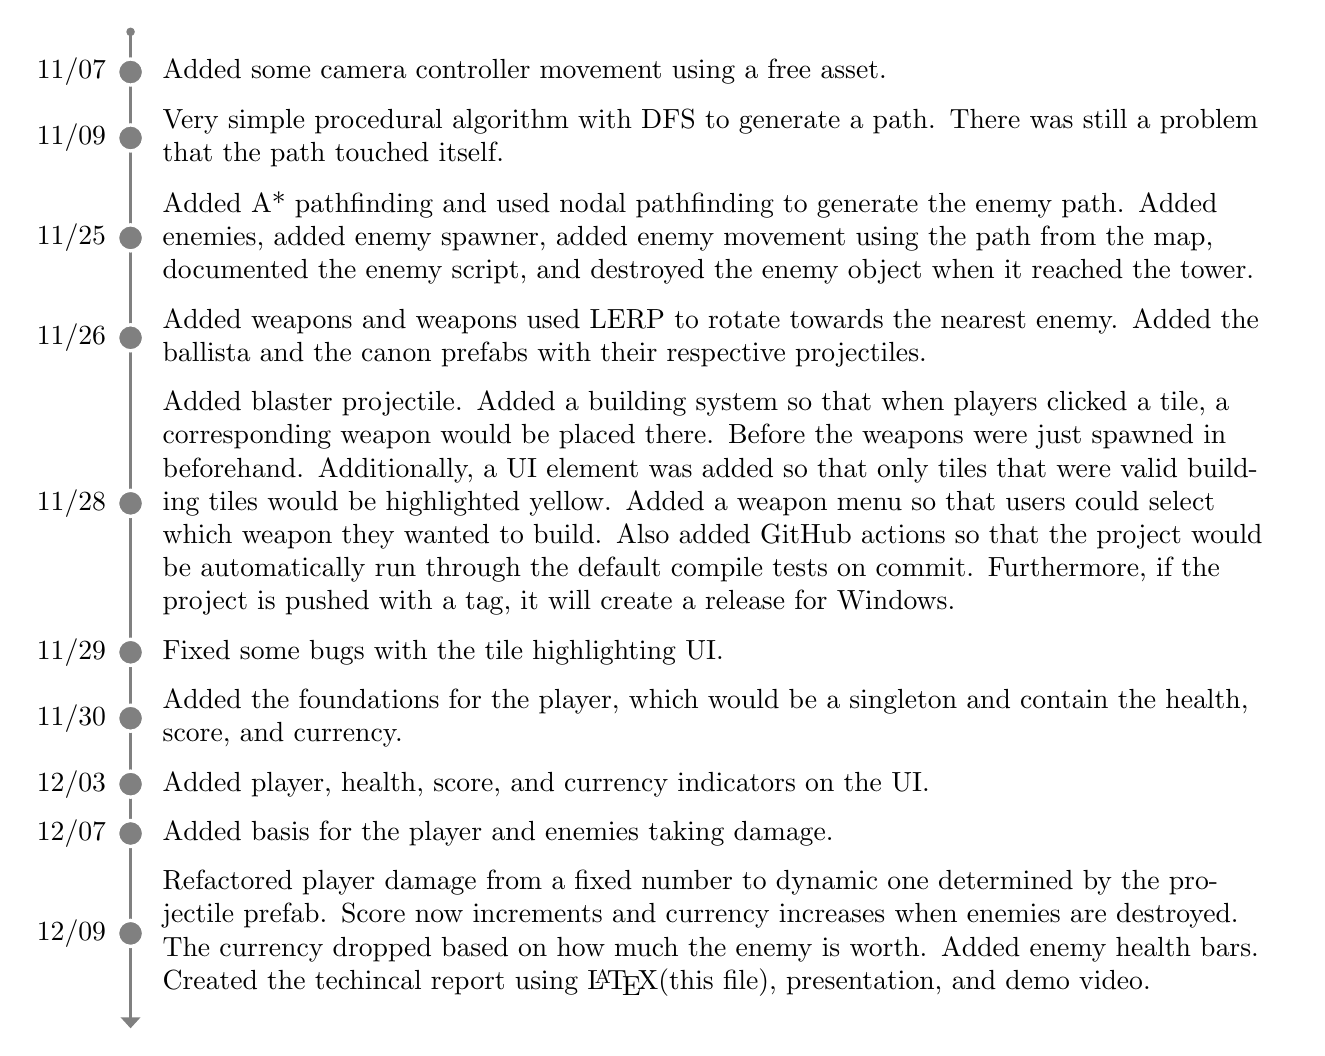
\begin{tikzpicture}[
        node distance = 1mm and 3mm,
        start chain = A going below,
        dot/.style = {
                circle,
                draw=white,
                very thick,
                fill=gray,
                minimum size=3mm,
            },
        box/.style = {
                rectangle,
                text width=140mm,
                inner xsep=4mm,
                inner ysep=1mm,
                on chain,
            },
    ]
    \begin{scope}[every node/.append style={box}]
        \node { Added some camera controller movement using a free asset. };
        \node { Very simple procedural algorithm with DFS to generate a path. There was still a problem that the path touched itself. };
        \node { Added A* pathfinding and used nodal pathfinding to generate the enemy path. Added enemies, added enemy spawner, added enemy movement using the path from the map, documented the enemy script, and destroyed the enemy object when it reached the tower. };
        \node { Added weapons and weapons used LERP to rotate towards the nearest enemy. Added the ballista and the canon prefabs with their respective projectiles. };
        \node { Added blaster projectile. Added a building system so that when players clicked a tile, a corresponding weapon would be placed there. Before the weapons were just spawned in beforehand. Additionally, a UI element was added so that only tiles that were valid building tiles would be highlighted yellow. Added a weapon menu so that users could select which weapon they wanted to build. Also added GitHub actions so that the project would be automatically run through the default compile tests on commit. Furthermore, if the project is pushed with a tag, it will create a release for Windows. };
        \node { Fixed some bugs with the tile highlighting UI. };
        \node { Added the foundations for the player, which would be a singleton and contain the health, score, and currency. };
        \node { Added player, health, score, and currency indicators on the UI. };
        \node { Added basis for the player and enemies taking damage. };
        \node { Refactored player damage from a fixed number to dynamic one determined by the projectile prefab. Score now increments and currency increases when enemies are destroyed. The currency dropped based on how much the enemy is worth. Added enemy health bars. Created the techincal report using \LaTeX (this file), presentation, and demo video. };
    \end{scope}
    \draw[very thick, gray,
    {Triangle[length=4pt)]}-{Circle[length=3pt]},shorten <=-3mm, shorten >=-3mm]
    (A-10.south west) -- (A-1.north west);
    \foreach \i [ count=\j] in {
            11/07,
            11/09,
            11/25,
            11/26,
            11/28,
            11/29,
            11/30,
            12/03,
            12/07,
            12/09
        }
    \node[dot,label=left:\i] at (A-\j.west) {};
\end{tikzpicture}

\section{Reflection}
\label{sec:Reflection}

% Insert Reflection Here %

\section{References}
\label{sec:References}

\begin{itemize}
    \item \href{https://youtu.be/ulFc6p3hQzQ}{3D Tilemap in Unity}
    \item \href{https://www.youtube.com/playlist?list=PLPV2KyIb3jR4u5jX8za5iU1cqnQPmbzG0}{Brackeys Unity Tower Defense}
    \item \href{https://forum.unity.com/threads/how-can-i-place-a-tile-in-a-tilemap-by-script.508338/}{Manual Tilemap Unity}
    \item \href{https://blog.unity.com/technology/procedural-patterns-you-can-use-with-tilemaps-part-i}{Procedural Tilemap}
    \item \href{https://www.kenney.nl/assets/tower-defense-kit}{Kenney Tower Defense}
    \item \href{https://isaacbroyles.com/gamedev/2020/07/04/unity-github-actions.html}{Unity GitHub Actions}
\end{itemize}

\end{document}